\section{Complete-time results for exact triangles and target batches}
\label{sec:notes-analytic-batch-results}
The reserved comparison contains forty native two-loop box requests, thirteen independent triangle products, one triangle with a symbolic scale, and four compatibility requests. Thirty-two box requests use fresh kinematics with the original index patterns, while eight use new index batches. The compatibility requests retain the earlier vacuum, propagator, and ladder definitions. Appendix~\ref{app:notes-analytic-batch} specifies every collection and the separation between training, validation, and testing.

Each measurement starts a fresh application process and includes loading, model use, exact reduction, retries, output, and the independent coefficient comparison. Three repetitions rotate method order on each request's worker. A first unverified result remains recorded and stops further repetitions for that method and request. Completed-time ratios include only requests verified by both compared methods; the separate completion table retains all requests.

The reserved measurements use two single-core workers on the same Intel(R) Xeon(R) Gold 6240 CPU @ 2.60GHz compute node. We fix that hardware assignment before the reserved tests. The full application validation uses a fresh profile on the same hardware. We preserve an interrupted heterogeneous-worker comparison in the notes; those trials do not determine admission. Each request compares every method on the same worker. The cluster allocation shares the node with other work, and the reported repetition intervals describe variation under those conditions.

Training selects 1 tree with maximum depth 4 and minimum leaf population 2. The full application validation takes 45.942 seconds with the selected policy and 49.598 seconds with the fixed action. Its time ratio is 0.926, with request-resampling interval $[0.853,0.995]$. The deployment rule therefore enables the new batch model. The separate reserved comparisons below measure the added learned choice after this decision.

The selected fixed action is the wider shared sparse region. The tree changes that action only when its predicted saving exceeds 8\% of the fixed cost plus 0.002 seconds. It changes the fixed action on 3 model-selection requests and makes a prediction on 38 reserved requests within its input ranges. Exact formulas and the preceding application handle the remaining structures or inputs outside those ranges.

Within those reserved predictions, the model selects the tighter shared sparse region on 7 requests and the wider shared sparse region on 31 requests. These observed choices show which alternatives contribute to the deployed result.

\begin{table}[!htbp]\centering\small
\caption{Complete-time comparison with the preceding application supplied with the same checked master indices. Times are sums of request medians in seconds. Each row uses only pairs that pass all three repetitions. A ratio below one means less time.}
\label{tab:notes-analytic-batch-times}
\begin{tabularx}{\linewidth}{@{}Yrrrr@{}}\toprule
Collection & Pairs & New & Same-basis control & Ratio\\\midrule
Planar box batches & 16 & 27.549 & 46.252 & 0.596 \\
Nonplanar box batches & 16 & 65.740 & 96.545 & 0.681 \\
New index batches & 8 & 35.722 & 44.213 & 0.808 \\
Triangle products, one to thirteen loops & 13 & 2.540 & 29.240 & 0.087 \\
Triangle with symbolic scale & 1 & 0.255 & 0.642 & 0.397 \\
Compatibility requests & 4 & 2.313 & 2.384 & 0.970 \\
All matched requests & 58 & 134.119 & 219.277 & 0.612 \\
\bottomrule\end{tabularx}\end{table}

Against the preceding method with the same basis, the final method uses 38.8\% less time on 58 matched requests. The ratio is 0.612, with repetition interval $[0.604,0.623]$. The new method is slower on 8 of those individual requests; the largest individual time ratio is 1.157. These per-request outcomes remain visible in the full result record.

Against the unmodified preceding application, the final method uses 67.6\% less time on 52 matched requests. The ratio is 0.324, with repetition interval $[0.321,0.331]$. The matched populations can differ because failed requests remain outside a completed-time ratio. Their totals therefore cannot be subtracted to assign a basis-preparation saving.

\begin{table}[!htbp]\centering\small
\caption{Added effect of the new batch decision on native requests. The fixed control has the same exact methods and basis, with the new model disabled. Both methods retain the preceding sparse expert where its action calls for it. These are original measurements of this study.}
\label{tab:notes-analytic-batch-ml}
\begin{tabularx}{\linewidth}{@{}Yrrrr@{}}\toprule
Collection & Pairs & Final time & Fixed time & Ratio\\\midrule
Planar box batches & 16 & 27.549 & 28.864 & 0.954 \\
Nonplanar box batches & 16 & 65.740 & 71.957 & 0.914 \\
New index batches & 8 & 35.722 & 31.725 & 1.126 \\
All native box batches & 40 & 129.010 & 132.546 & 0.973 \\
\bottomrule\end{tabularx}\end{table}

Against the fixed batch action over the forty native box requests, the final method uses 2.7\% less time on 40 matched requests. The ratio is 0.973, with repetition interval $[0.962,0.989]$. This subtotal isolates the added model on the native workload. The full-workflow comparisons below also retain exact and compatibility requests.

The learned choice takes more time on 19 individual native requests, with a largest request ratio of 2.386. Its aggregate saving therefore does not imply a saving for each input. The recorded native elimination counters total 3,155,328 operations for the learned choice and 3,449,687 for the fixed action. These counters cover the instrumented native algebra; they exclude loading, symbolic checks, and direct-formula arithmetic. The complete timer includes those costs.

Against the same workflow with a fixed batch action, the final method uses 2.5\% less time on 58 matched requests. The ratio is 0.975, with repetition interval $[0.961,0.994]$. Against the same workflow with both learned choices disabled, the final method uses 1.9\% less time on 58 matched requests. The ratio is 0.981, with repetition interval $[0.972,0.999]$. The second control changes the earlier seed choice as well, so its difference measures the combined learned decisions.

\begin{figure}[!htbp]\centering
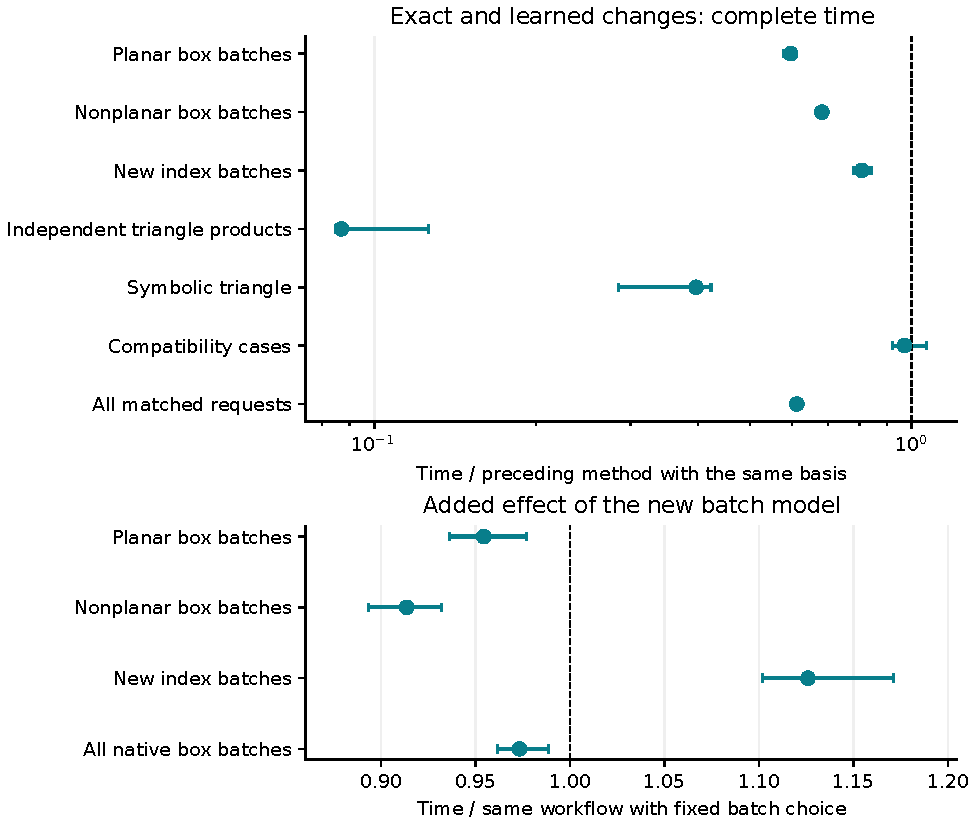
\includegraphics[width=\linewidth]{paper_figures/analytic_batch.pdf}
\caption{The upper panel measures the combined analytic and learned changes with matched basis preparation. Its logarithmic axis accommodates the exact-triangle saving and the smaller native changes. The lower panel isolates the new batch choice within the native test groups. Horizontal intervals describe paired repetition variation. The line at one indicates equal time; completion counts appear separately in Table~\ref{tab:notes-analytic-batch-completion}.}
\label{fig:notes-analytic-batch}
\end{figure}
\begin{table}[!htbp]\centering\small
\caption{Completion and first-pass cost over all 58 reserved requests. A verified request must pass all three repetitions. First-pass time sums the first measured application and check cost for every request, including failed work. The paired completed-time ratios appear in Table~\ref{tab:notes-analytic-batch-times}.}
\label{tab:notes-analytic-batch-completion}
\begin{tabularx}{\linewidth}{@{}Yrrr@{}}\toprule
Method & Verified & First unverified & First-pass seconds\\\midrule
Final method & 58 & 0 & 135.430 \\
Fixed batch action & 58 & 0 & 139.245 \\
Both learned choices disabled & 58 & 0 & 137.895 \\
Preceding method, same basis & 58 & 0 & 220.267 \\
Unmodified preceding application & 52 & 6 & 597.327 \\
\bottomrule\end{tabularx}\end{table}

The reserved test contains 858 measured outcomes and 14,226 successful coefficient comparisons. The added basis preparation takes 15.747 seconds and supplies 126 coefficient checks across five development requests. Independent reference preparation for the reserved set takes 237.539 seconds. These one-time and benchmark costs remain separate from the supplied-basis totals. The stored master indices contain no solved target coefficients.

Training-data collection, model selection data, and full-cost admission use 1663.451 seconds of summed measured application time. Their independent references add 261.918 seconds. These are separate one-time learning costs. The reserved reduction times measure use of the prepared method and do not imply that training has already paid for itself in a single calculation. Summed process times also differ from elapsed collection time when two workers run concurrently.

The triangle identity has an explicit analytic domain and independent native checks. The learned model has a narrower measured domain: two massless two-loop box structures with rational kinematics and symbolic dimension. The new index batches test transfer within those structures. General connected higher-loop scattering and all integral types remain outside this evidence. A finite candidate search also cannot prove that the selected workflow has the smallest possible runtime.
\FloatBarrier
\subsection{Preserved validation before the hardware assignment}
The initial full application validation used profile $3037$ on two different cluster nodes. It recorded 79 completed measurements with exact agreement before the slower worker was stopped. Their summed measured time is 606.267 seconds. The runtime and measurement sources, completed records, and interrupted inputs remain preserved. These measurements do not enter the admission decision. We retain the selected tree and its weights, then use the fresh profile $3041$ on the fixed reserved-test node for the completed validation. This change precedes all reserved testing and changes no target reduction formula.
